% --------------------------
% ---- DECLARE PACKAGES ----
% --------------------------
\documentclass[a4paper, oneside, openright]{book}
\usepackage[T1]{fontenc} % Font encoding, T1 = it
\usepackage{lmodern}
\usepackage{booktabs}
\usepackage{multicol} % Per il frontespizio
\usepackage[utf8]{inputenc} % Input encoding - per caratteri particolari
\usepackage[english]{babel} % Lingua principale italiano, con parti in inglese
\usepackage{blindtext} % Per la generazione di paragrafi lorem ipsum
\usepackage{graphicx} % Per includere immagini esterne
\usepackage[a4paper,top=2.5cm,bottom=2.5cm,left=3cm,right=3cm]{geometry} %impaginazione e margini documento
\usepackage[fontsize=13pt]{scrextend} %dimensione font
\usepackage{graphicx}
\usepackage[parfill]{parskip} % Disabilita l'indentazione dopo essere andati a capo
% \usepackage[hang,flushmargin]{footmisc} % Disabilita l'indentazione nelle footnotes
\usepackage{titlesec}

\usepackage{minted} % Per i blocchi di codice
\usepackage{float}
\usepackage{amsmath} % For advanced math typesetting
\usepackage{amssymb} % For additional symbols, if needed
\usepackage{graphicx} % For including figures, if applicable
\usepackage[font=scriptsize, skip=5pt]{caption} % Spazio tra la caption e l'immagine
\usepackage[backend=biber, style=numeric, backref=true,defernumbers=true]{biblatex}
\usepackage[immediate]{silence}
\WarningFilter[temp]{latex}{Command} % silence the warning
\usepackage{sectsty}
\DeactivateWarningFilters[temp] % So nothing unrelated gets silenced
\usepackage{hyperref} % Rende l'indice cliccabile
\usepackage[justification=centering]{caption} % Per centrare le captions
\usepackage{csquotes} % Dipendenza di babel
\usepackage[bottom]{footmisc} % Posiziona le footnotes alla fine della pagina
\usepackage{hyperref}
\usepackage{enumitem}
\usepackage{amsmath, amssymb, graphicx}
\usepackage{hyperref}
\newcommand{\cmark}{\ding{51}}  % checkmark
\newcommand{\xmark}{\ding{55}}  % x-mark
\usepackage{pifont}
\bibliography{references}        % no .bib extension!



% ------------------------
% ---- DOCUMENT SETUP ----
% ------------------------
\pagestyle{plain}
\raggedbottom % Se la pagina non è completa, lascia lo spazio alla fine

\titleformat{\chapter}[display]
    {\normalfont\huge\bfseries}{}{0pt}{\LARGE} % Remove chapter number display
\titlespacing*{\chapter}{0pt}{0pt}{20pt} 
\chaptertitlefont{\fontsize{22pt}{30pt}\selectfont}

\hypersetup{ % Setup dell'aspetto dei link
    colorlinks,
    citecolor=black,
    filecolor=black,
    linkcolor=black,
    urlcolor=black
}

% \renewcommand{\footnoterule}{ % Rende la linea delle footnotes larga tutta la pagina
%   \kern -3pt
%   \hrule width \textwidth height 1pt
%   \kern 2pt
% } 
\renewcommand{\footnotesize}{\fontsize{11pt}{13pt}\selectfont} % Imposta la dimensione del testo delle footnotes
\setlength{\footnotesep}{0.5cm} % Imposta lo spazio fra e singole footnotes
\setlength{\skip\footins}{1.5cm} % Imposta lo spazio fra il corpo e le footnotes

\DeclareUnicodeCharacter{02BC}{}

% ------------------------
% ---- DOCUMENT START ----
% ------------------------
\addbibresource{bibliography.bib} % Importiamo la bibliografia
\begin{document} % Inizio documento
\pagenumbering{gobble} % Disabilita numerazione pagine
\begin{titlepage}
\begin{figure}[!htb]
    \centering
    
\includegraphics[width=8cm]{Images/Logo_Politecnico_Milano.png}
\end{figure}

\begin{center}
    \LARGE{\textbf{POLITECNICO DI MILANO}} \\[2mm]
    
    \small{\textbf{MASTER'S PROGRAM IN}} \\[1mm]
    
    \small{\textbf{HIGH PERFORMANCE COMPUTING ENGINEERING}} \\[2mm]
\end{center}

\vspace*{\fill}

\begin{center}
    \Large{\textbf{High-Performance Parallel Implementation of the Susceptible-Infected-Recovered (SIR) Epidemic Model using MPI and Runge-Kutta Numerical Integration}}\\
\end{center}

\vspace*{\fill}

\begin{minipage}[t]{1\textwidth}
    \vspace{-10mm}
    {\small \textbf{Group Members:}}\\[2mm]
    {\small
    Milica Sanjevic \hfill Person Code: 10975337\\
    Salvatore Mariano Librici \hfill Person Code: 11078653\\
    Yibo Li \hfill Person Code: 11022291\\
    Nada Elsayed \hfill Person Code: 10998973\\
    Hirdesh Kumar \hfill Person Code: 10997383\\
    }
\end{minipage}



\vspace{10mm}

\begin{center}
    {\small{\textbf{Academic Year:}}{\small\vspace{0.5mm}
    \\ \small{2024/2025}}}  
\end{center}

\end{titlepage}
 % PAGINA FRONTESPIZIO

\pagenumbering{arabic} % Riabilita la numerazione in modo che cominci dal primo capitolo
\setcounter{chapter}{1} % Fa risultare l'introduzione come capitolo 0
% ------------------
% ---- CHAPTERS ----
% ------------------
\tableofcontents  % Genera l'indice


\newpage
\textbf{Abstract}:  
This project presents a parallel simulation framework based on the classical SIR (Susceptible-Infected-Recovered) epidemic model, aimed at studying the dynamics of disease spread in spatially structured populations. The model discretises the simulation domain into a 2D grid where each cell evolves over time according to the SIR equations. To ensure numerical accuracy, the system is integrated using the 4th-order Runge-Kutta method. For scalability, the implementation employs MPI-based domain decomposition and ghost cell exchange, allowing the simulation to run efficiently across multiple processors. Experimental results validate the correctness and performance of the framework, and the architecture is designed to be extensible for other spatial epidemic or information propagation scenarios.

\section{Introduction}

Modeling the spread of diseases across spatial domains is an important task in computational epidemiology. Classical compartmental models, such as the SIR (Susceptible-Infected-Recovered) model, capture population-level transitions between health states, but often assume a well-mixed population. In reality, geographic and social structures cause spatial heterogeneity, making grid-based modeling more appropriate for certain applications.

In this work, we simulate the SIR model over a two-dimensional spatial grid, where each cell represents a subregion of the population. The infection dynamics are governed by ordinary differential equations, which are numerically solved using a 4th-order Runge-Kutta (RK4) integration scheme to ensure accuracy and stability.

To enable high-resolution and large-scale simulations, we parallelize the framework using the Message Passing Interface (MPI). The spatial domain is decomposed across MPI ranks, and ghost cell communication is used to preserve local interaction at region boundaries. The simulation is implemented in C++, and performance evaluations confirm its scalability and balanced workload distribution across ranks.

We adopt MPI to support distributed memory parallelism, which is essential for scaling to large domains and executing the simulation efficiently on multi-node systems.

Although this work focuses on infectious disease modeling, the underlying architecture can be generalized to simulate other types of spatial propagation processes, such as information diffusion or network congestion, making it a versatile foundation for future research.

\section{Background and Definitions}

\paragraph{Grid Structure and Neighborhoods.}
The simulation domain is discretized into a two-dimensional grid, where each cell represents a subregion of the population. For each cell, we define a neighborhood consisting of the adjacent cells (typically using the 4-neighbor or 8-neighbor scheme) to model spatial interactions in the infection dynamics.

\paragraph{Ghost Cells and Parallelization.}
In the MPI-based parallel implementation, the grid is partitioned across multiple ranks. To maintain data consistency at subdomain boundaries, we use ghost cells—copies of neighboring cells from adjacent ranks—which are updated through inter-process communication at each time step.

\paragraph{Single Cell Evolution.}
Each simulation cell independently evolves over time according to the SIR model's ordinary differential equations (ODEs). The evolution is computed using a 4th-order Runge-Kutta (RK4) method for numerical integration. In the parallel version, each RK4 step incorporates values from neighboring cells via ghost cell communication to model spatial infection spread.



\newpage
\section{Mathematical Formulation}
We adopt the classical SIR (Susceptible–Infected–Recovered) model to simulate the dynamic evolution of states within a spatial grid. Each grid cell maintains the proportion of its population in the three states:

\begin{itemize}
    \item \textbf{S}: Susceptible individuals
    \item \textbf{I}: Infected individuals
    \item \textbf{R}: Recovered individuals
\end{itemize}

The local dynamics of state transitions are governed by the standard system of differential equations:

\begin{align*}
\frac{dS}{dt} &= -\beta S \cdot I \\
\frac{dI}{dt} &= \beta S \cdot I - \gamma I \\
\frac{dR}{dt} &= \gamma \cdot I
\end{align*}

To model spatial interaction across neighboring cells, we extend the equations by incorporating a coupling term that accounts for the influence of infected populations in adjacent locations. The modified equation for the susceptible population in cell \((i, j)\) becomes:

\[
\frac{dS_{ij}}{dt} = -\beta S_{ij} \cdot \left( I_{ij} + \sum_{(k,l) \in N(i,j)} I_{kl} \right)
\]

where \( N(i,j) \) denotes the set of neighboring cells of \((i,j)\). Similar formulations are used for \( \frac{dI_{ij}}{dt} \) and \( \frac{dR_{ij}}{dt} \) to capture spatially distributed SIR dynamics.


\newpage
\section{Numerical Methods}
We employ a 4th-order Runge-Kutta (RK4) integrator for each time step to solve the system of ordinary differential equations governing the state transitions.\cite{butcher2003numerical} This method offers a good balance between computational efficiency and numerical accuracy, making it well-suited for time-dependent simulations of interacting systems. Compared to simpler schemes such as Euler’s method, RK4 significantly reduces error accumulation over long-term integration.

Each cell’s state—represented by the fractions of susceptible (S), informed (I), and blocked (R) vehicles—is updated based on both local values and the influence from neighboring cells. To achieve this, we implement a neighbor-aware RK4 variant in the function \texttt{rk4StepWithNeighbors()}, which calculates intermediate derivatives using the average infected fraction from adjacent cells. This allows the simulation to realistically capture the spatial diffusion of information or congestion.

After each RK4 update, we apply a normalization step to ensure that the sum \( S + I + R = 1 \), preserving the physical consistency of the model. This normalization also helps prevent numerical drift due to floating-point approximations across iterations.



\newpage
\section{Code Architecture and Structure}
\begin{figure}[!htb]
    \centering
    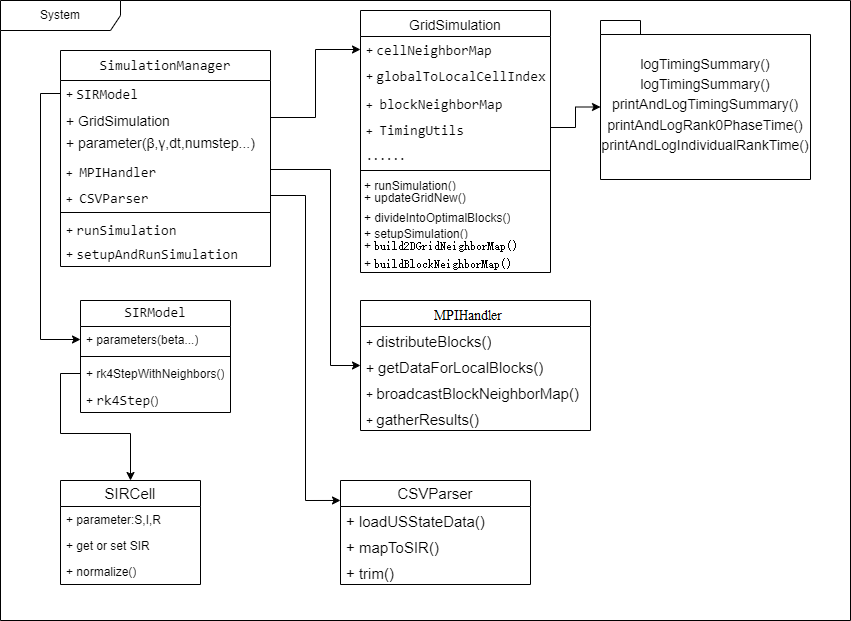
\includegraphics[width=12cm]{Images/pic0.png}
\end{figure}


\subsection{CSVParser Class}
The \texttt{CSVParser} class is responsible for reading and preprocessing real-world COVID-19 data from CSV files. It extracts relevant fields such as population, confirmed, recovered, and active cases, and converts them into normalized SIR values. The parsed data is returned as \texttt{SIRCell} instances, ensuring that each cell satisfies \( S + I + R = 1 \) through internal normalization.


\subsection{SIRCell Class}
This class encapsulates the state variables of each simulation cell: susceptible (S), infected (I), and recovered (R). It provides getter and setter methods with bounds checking to ensure physical validity.  
After each update, we apply a \texttt{normalize()} method that rescales the values so that \( S + I + R = 1 \).  

This normalization is not part of the classical SIR model itself, but a design choice introduced in our implementation to mitigate numerical drift and maintain probabilistic consistency.


\subsection{SIRModel Class}
The \texttt{SIRModel} class defines the evolution equations and implements two versions of the Runge-Kutta 4th-order integration: one for isolated cells, and one that incorporates neighbor influence (\texttt{rk4StepWithNeighbors}). It holds model parameters such as \( \beta \), \( \gamma \), timestep size, and total number of steps.

\subsection{GridSimulation Class}
This class is responsible for managing the entire simulation grid, including the local cells, global-to-local ID mappings, and ghost regions. It handles the step-by-step evolution of the system, sets up the neighbor relations, and maintains grid partitioning and block ownership across ranks.

\subsection{TimingUtils}
The \texttt{TimingUtils} provides utility functions for logging and analyzing the runtime performance of the simulation. It records the execution time of each phase (e.g., initialization, communication, computation) across all MPI ranks. The class supports generating both global and rank-specific timing summaries, including minimum, maximum, and average statistics. This data helps identify bottlenecks and evaluate the scalability of the simulation framework.

\subsection{MPIHandler and SimulationManager Classes}
The \texttt{MPIHandler} class abstracts all MPI-related communication, including distributing grid blocks, exchanging ghost cells, and gathering final results. The \texttt{SimulationManager} class coordinates the entire simulation workflow: loading data, initializing components, running the main loop, and storing output.

\subsection{Design Principles and Code Organization}
The code is structured with modularity and scalability in mind. Core logic is separated from communication routines, and all timing-related functionality is encapsulated in a utility module. The design ensures clear responsibility separation and allows easy testing or extension (e.g., for other ODE models or input formats).


\newpage
\section{Parallelization Techniques and Implementation}

\subsection{Parallelization with MPI}
To achieve scalable simulation of information and congestion propagation on large-scale smart road systems, this project employs the Message Passing Interface (MPI) to distribute the computational workload across multiple processors. Each processor (MPI rank) is responsible for evolving a subset of the overall grid representing spatial regions (e.g., states or road cells). Inter-process communication is used to exchange boundary (ghost) cells, enabling accurate interaction across adjacent regions.

MPI was selected due to the following advantages:
\begin{itemize}
    \item \textbf{Scalability}: MPI allows distributing computation across multiple cores and nodes, making it suitable for simulating large grids (e.g., 50+ cells).
    \item \textbf{Explicit communication}: As our model requires interaction between neighboring cells, MPI’s explicit control over data exchange provides both flexibility and performance.
    \item \textbf{Process isolation}: Each process handles only its assigned cells, reducing memory contention and increasing cache efficiency.
\end{itemize}

\subsubsection*{MPI Parallelization Workflow}
The main simulation procedure using MPI consists of the following steps:
\begin{enumerate}
    \item \textbf{Grid Partitioning (Rank 0)}: The global grid is first mapped using a cell ID mapping loaded from a CSV dataset. The function\\\texttt{divideIntoOptimalBlocks()} chooses the most balanced partitioning scheme. Cells are grouped into blocks and assigned to ranks.
    
    \item \textbf{Initial Communication}: Rank 0 broadcasts:
    \begin{itemize}
        \item Block-to-rank map
        \item Cell neighbor relationships
        \item Ghost neighbor relationships
    \end{itemize}
    Each rank initializes its local SIRCell grid using \texttt{setGridFromLocalData()}.

    \item \textbf{Ghost Cell Communication}: During each time step, ghost boundary cells are exchanged using non-blocking MPI operations:
    \begin{itemize}
        \item \texttt{MPI\_Isend} and \texttt{MPI\_Irecv} transfer S, I, R values to/from neighboring ranks.
        \item \texttt{MPI\_Barrier} ensures synchronization.
        \item Mapping from local index $\rightarrow$ global ID and global ID $\rightarrow$ owner rank is used to build send/receive buffers.
    \end{itemize}

    \item \textbf{Local Update}: Each cell is updated using \texttt{rk4StepWithNeighbors()}, incorporating the influence of both local and ghost neighbors. A normalization step ensures \( S + I + R = 1 \) for every cell.

    \item \textbf{Result Collection}: At the end of the simulation, each rank outputs its local average S, I, R to a time-series vector. Optionally, Rank 0 gathers global results for visualization.
\end{enumerate}

\subsection{MPI Functionality Highlights}
To understand performance behavior and potential bottlenecks, we conducted fine-grained timing analysis across different phases. Each rank logs the time spent in key MPI-related sections using a custom timing utility module\\ (\texttt{TimingUtils.cpp}). This provides rank-specific insights into load balancing and communication overhead.

\begin{table}[h]
\centering
\begin{tabular}{|l|p{9cm}|}
\hline
\textbf{Phase} & \textbf{Description} \\
\hline
\texttt{distributeBlocks()} & Initial grid partitioning on rank 0 \\
\texttt{Total\_MPI\_Prep\_In\_Loop\_RankX} & Time preparing ghost data buffers per step \\
\texttt{Total\_MPI\_Comm\_In\_Loop\_RankX} & Actual non-blocking send/receive time \\
\texttt{Total\_Local\_Computation\_RankX} & RK4 updates using local + ghost values \\
\texttt{runSimulation\_TotalWallTime} & Overall simulation time (barrier-to-barrier) \\
\hline
\end{tabular}
\caption{MPI Timing Categories}
\end{table}

We observed that computation dominates total execution time, but MPI communication becomes significant as the number of ranks increases.
\begin{figure}[!htb]
    \centering
    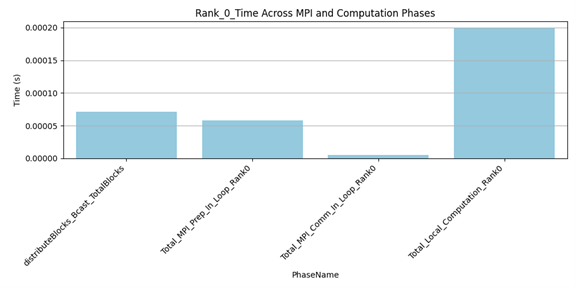
\includegraphics[width=14cm]{Images/pic1.png}
\end{figure}

\subsection{Visualization of Spatial Communication}
To explore the impact of rank-based spatial decomposition, we visualize the evolution of infection intensity per rank over time. Each MPI rank controls a specific grid region (e.g., a block of US states), and infection spreading dynamics are influenced by local conditions and ghost exchange.

Key observations:
\begin{itemize}
    \item Some ranks remain uninfected due to lack of spatial contact (e.g., isolated blocks).
    \item Peak infection times vary across ranks due to asynchronous propagation.
\end{itemize}
\begin{figure}[!htb]
    \centering
    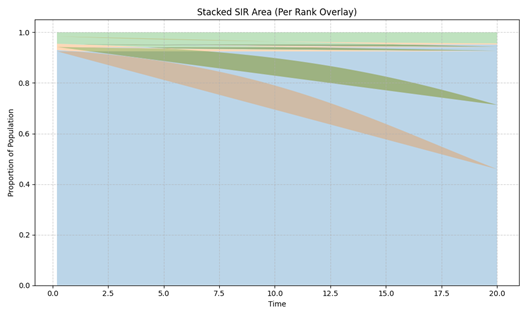
\includegraphics[width=14cm]{Images/pic3.png}
    
\end{figure}\begin{figure}[!htb]
    \centering
    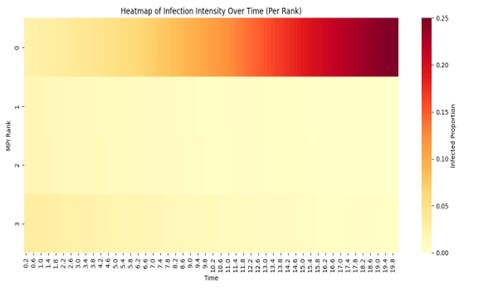
\includegraphics[width=14cm]{Images/pic2.jpg}
\end{figure}
\subsection{Performance Results and Scalability}
We compared execution time across configurations (e.g., 4 ranks, 8 ranks). As expected, total wall time decreases with more ranks, up to a limit. Communication overhead grows superlinearly due to ghost cell exchange.

\textbf{Observations}:
\begin{itemize}
    \item For 4 ranks, communication is negligible compared to computation.
    \item Communication overhead grows with process count.
    \item Load balancing is maintained via \texttt{divideIntoOptimalBlocks()}.
\end{itemize}
\begin{figure}[!htb]
    \centering
    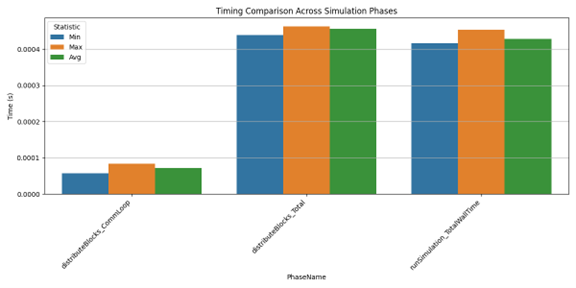
\includegraphics[width=14cm]{Images/pic4.png}
\end{figure}
\subsection{Summary of parallel implementation}
The MPI-based simulation achieves efficient spatial parallelization of the SIR model by distributing blocks of the grid across multiple processes. Each MPI rank is responsible for computing a subset of the grid, and ghost cells are exchanged between neighboring ranks to ensure correct interactions at boundaries.

This parallel structure reduces computation time significantly for large grids while preserving accuracy in local dynamics through explicit message passing. The simulation is organized in a modular fashion, separating responsibilities for grid partitioning, communication, and local updates, which improves code maintainability and profiling capabilities.


\newpage
\section{Experimental Setup}

\subsection{Input Data}
The simulation is initialized using real-world data derived from U.S. COVID-19 state-level daily reports, published by the Johns Hopkins CSSE dataset. Each record corresponds to a U.S. state and includes epidemiological and demographic features.

Before integration, the raw data is cleaned and preprocessed using Python scripts (\texttt{clean\_sort\_dataset.py}). The resulting CSV files contain:
\begin{itemize}
    \item \texttt{Province\_State}: Name of the U.S. state
    \item \texttt{Population}: Total number of residents in the state
    \item \texttt{Lat, Long}: Geographic coordinates
    \item \texttt{Confirmed, Deaths, Recovered}: Historical COVID-19 case data
    \item Derived S, I, R values based on these statistics
\end{itemize}

Each file is reformatted with consistent headers and column ordering. Missing values are filled using backward filling or known approximations. The data is sorted geographically to preserve adjacency relationships in the simulation grid.

\textbf{Example files}: \texttt{sorted\_01-01-2021.csv}, \texttt{sorted\_02-05-2021.csv}

\subsection{Simulation Parameters}
We test the model under various combinations of infection rate \( \beta \) and recovery rate \( \gamma \) to reflect different behavioral and traffic conditions. These parameters mirror classical SIR dynamics:
\begin{itemize}
    \item \( \beta \): Controls how fast information spreads among vehicles
    \item \( \gamma \): Reflects how quickly congestion is resolved
\end{itemize}

\begin{table}[h]
\centering
\begin{tabular}{|c|c|c|l|}
\hline
\textbf{Scenario} & \( \beta \) & \( \gamma \) & \textbf{Interpretation} \\
\hline
Baseline & 0.3 & 0.1 & Moderate info spread and recovery \\
Fast Spread & 0.5 & 0.1 & Aggressive dissemination of signals \\
Fast Recovery & 0.3 & 0.3 & Faster clearing of blocked roads \\
Low Transmission & 0.1 & 0.1 & Weak signal sharing; slow dynamics \\
\hline
\end{tabular}
\caption{Tested parameter scenarios}
\end{table}

Each configuration simulates 20 iterations using a fixed time step of \( \Delta t = 0.2 \).


\newpage
\section{Results and Analysis}

\subsection{Accuracy and Model Behavior}
The model enforces the constraint \( S + I + R = 1 \) at every grid cell and time step, ensuring physical consistency and mitigating numerical drift due to floating-point errors. This is achieved via post-integration normalization.

Across all scenarios, the model exhibits expected qualitative behaviors:
\begin{itemize}
    \item \textbf{Higher \( \beta \)}: Faster and broader propagation; earlier infection peaks
    \item \textbf{Higher \( \gamma \)}: Rapid decline in infections; quicker recovery
    \item \textbf{Low \( \beta + \gamma \)}: Slower dynamics; longer persistence of initial state
\end{itemize}

These trends confirm that the simulation is sensitive to parameters and effectively captures distributed information and congestion dynamics.

\subsection{Visualization}

\subsubsection{Global SIR Evolution}
We first provide an overview of the global trends of the SIR variables:
\begin{figure}[H]
    \centering
    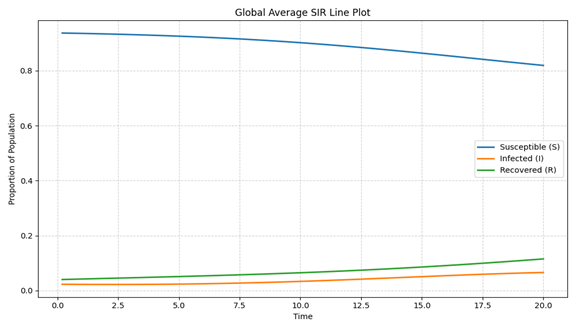
\includegraphics[width=14cm]{Images/pic5.png}
    \caption*{Shows the global average values of Susceptible (S), Infected (I), and Recovered (R) over time, plotted as line graphs. It confirms the expected dynamics: S steadily decreases, while I and R gradually increase.}
    \label{fig:sir_line_plot}
\end{figure}

\begin{figure}[H]
    \centering
    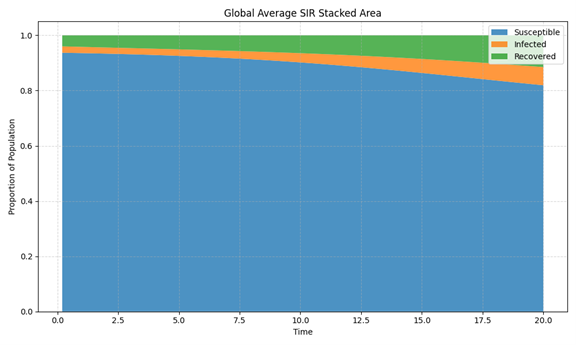
\includegraphics[width=14cm]{Images/pic6.png}
    \caption*{Presents the same data in the form of a stacked area chart, emphasizing the total population conservation (S + I + R = 1) and the proportion each state occupies throughout the simulation.}
    \label{fig:pic6}
\end{figure}


\subsubsection{Per-Rank Behavior}
Because the simulation is distributed across MPI processes, it is important to visualize the behavior of each rank individually.
\begin{figure}[H]
    \centering
    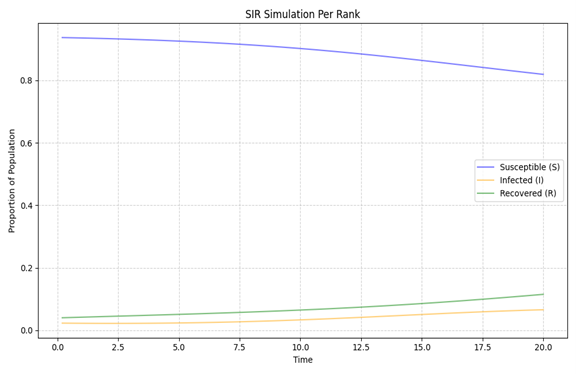
\includegraphics[width=14cm]{Images/pic7.png}
    \caption*{Displays the evolution of S, I, and R within each MPI rank using line plots. These trends reveal differences in infection dynamics between regions, reflecting the spatial heterogeneity.}
    \label{fig:sir_line_plot}
\end{figure}

\subsubsection{Infection Propagation and Peak Timing}
To analyze the infection wave’s temporal spread and communication among ranks:
\begin{figure}[H]
    \centering
    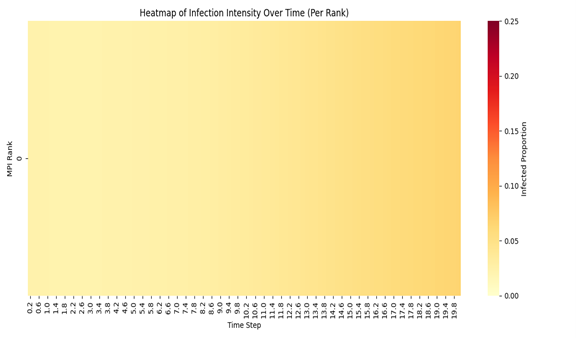
\includegraphics[width=14cm]{Images/pic8.png}
    \caption*{This is a heatmap that illustrates the infection intensity per rank over time. It demonstrates how the infection begins locally and gradually spreads to other ranks through the ghost cell exchange mechanism.}
    \label{fig:sir_line_plot}
\end{figure}

\subsection{Performance and Scaling Analysis}
Based on the results presented in Section 7.2, we evaluate the parallel simulation’s computational efficiency. The recorded timing logs, including phase-specific breakdowns and rank-level measurements, confirm that the workload is well-balanced across MPI processes. Most of the execution time is spent in the local computation phase, while communication costs remain relatively low due to the use of non-blocking MPI operations.


The distribution of timing across ranks shows minimal variability, indicating that the domain decomposition strategy (divideIntoOptimalBlocks) effectively assigns cells to processes with balanced loads. The asynchronous communication scheme using MPI\_Isend and MPI\_Irecv overlaps well with computation, helping to reduce idle time during ghost cell exchange.



\newpage
\section{Conclusion and Future Work}


We successfully implemented a high-performance parallel simulation framework that extends the classical SIR (Susceptible-Infected-Recovered) model to simulate smart road dynamics. The focus of this project was not on fully achieving smart road functionality, but rather on constructing a modular and scalable proof-of-concept system that demonstrates the feasibility of adapting epidemic modeling to spatially distributed vehicle networks. The model leverages 4th-order Runge-Kutta numerical integration and MPI-based parallelization with ghost cell synchronization to support large-scale simulations.

The system has shown accurate behavior, stable performance, and strong scaling properties. Timing analysis confirms efficient distribution of computational load, and visualization validates the consistency of infection dynamics across partitions.

Looking forward, several directions can further enhance the model’s realism and applicability. One avenue is the incorporation of directional vehicle flow to better mimic real-world traffic behavior. Another key improvement is the use of dynamic load balancing techniques to adaptively distribute work among MPI ranks, particularly under spatially heterogeneous conditions. Additionally, the model can benefit from GPU acceleration through frameworks such as OpenACC or CUDA, which would further boost scalability. Integration with real-time sensor networks represents another valuable extension, enabling more responsive and data-driven simulations applicable to intelligent transportation systems.

This project lays a solid foundation for future research and development in parallel simulation of cyber-physical infrastructures.




\printbibliography




% ----------------------
% ---- DOCUMENT END ----
% ----------------------
\end{document} % Fine documento
